\chapter{Installing OpenFOAM and Paraview}
\thispagestyle{empty}
\label{sec:chap1}
\newcommand{\LocCHonefig}{\Origin/CHAPTERS/chap1/figures}

The First chapter deals with Installing OpenFOAM and Paraview. We are using Linux Operating System for installation and OpenFOAM-2.3.0 and Paraview-4.1.0.
First we will look how to install OpenFOAM and paraview using Synaptic Package Manager. Then using the downlading it from the OpenFOAM website and lastly installing
it using the source code. We will end this chapter with an example which shows running a simple problem in .As a basic requirement the user expected to have 
some basic knowledge of Computational Fluid Dynamics ( CFD ) and should be able to use basic Linux Commands.

\section{Installation using Synaptic Package Manager}

OpenFOAM and Paraview can be installed using Synaptic Package Manager. On the left side of your computer screen you can see the Launcher with the list of softwares.
Click on the search box ,Fig.\ref{search} on top of the Launcher and type Synaptic. This will display the Synaptic Package Manager. Click on it to open.

\begin{figure}[h]  
\begin{center}  

\includegraphics[scale=0.75]{\LocCHonefig/dash.png}
\caption{Search Icon on top of Launcher}
\label{search}
\end{center}  
\end{figure}

\flushleft You will be interrupted to enter the system password.

\begin{figure}[h]  
\begin{center}  
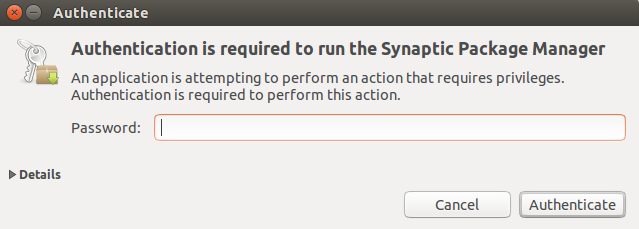
\includegraphics[scale=0.45]{\LocCHonefig/password.png}
\caption{Enter system password to open Synaptic Package Manager}
\end{center}  
\end{figure}
\vspace{1cm}

\flushleft Once the Synaptic Package Manager is Opened, in the search box type OpenFOAM.

\begin{figure}[ht]  
\begin{center}  
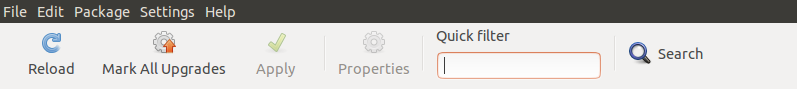
\includegraphics[scale=0.4]{\LocCHonefig/searchbox.png}
\caption{Search Box}
\label{searchbox}
\end{center}  
\end{figure}

\flushleft You will see both OpenFOAM-2.3.0 and Paraview-4.1.0. Right Click Both of them for installation and click Apply to install, Fig \ref{searchbox}. 
This might take some time to install depending upon your internet speed.

\begin{figure}[ht]  
\begin{center}  
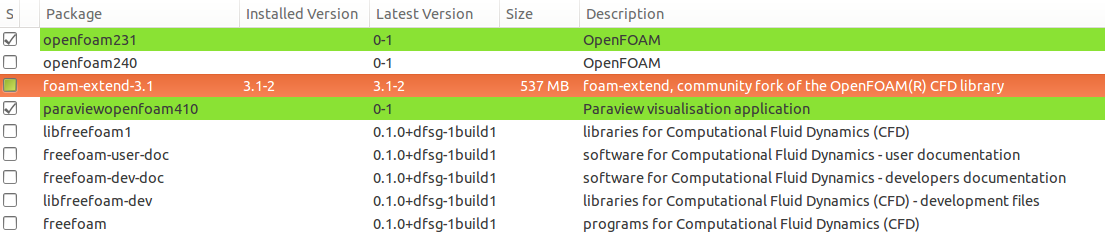
\includegraphics[scale=0.35]{\LocCHonefig/mark.png}
\caption{Install OpenFOAM and Paraview}
\label{searchbox}
\end{center}  
\end{figure}

\section{Installtion from OpenFOAM website}

\flushleft OpenFOAM can also be downloaded and installed using the OpenFOAM website. Follow the steps given below for installation. 
\begin{itemize}
\item On your browser type \textbf{www.openfoam.com/download} 
\item Go to Ubuntu Debian Installation
\item Under the first point of Installation copy the command line and paste this in your terminal window
\item Open the terminal window by pressing \textbf{Ctl+Alt+t} keys simultaneously on your keyboard or you can also open it using the 
search icon on top of the Launchbar

\begin{figure}[ht]  
\begin{center}  
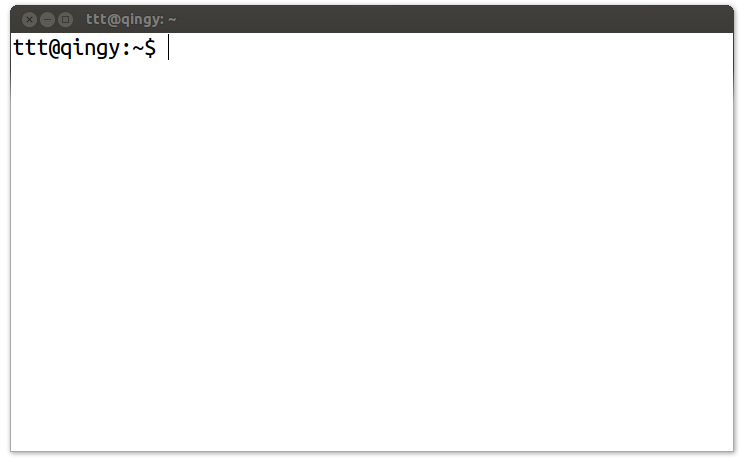
\includegraphics[scale=0.28]{\LocCHonefig/terminal.png}
\caption{Terminal window}
\label{terminal}
\end{center}  
\end{figure}

\item For complete installation for OpenFOAM and Paraview follow the steps under Ubuntu installation page

\end{itemize}

\flushleft To configure the installed software we need to edit the bashrc file. 
To do this open a new command terminal and type 
\begin{equation*}
\textbf{gedit $\sim$$\slash$.bashrc} 
\end{equation*}
and press enter

\flushleft After the bashrc file is opened scroll down to the bottom of the file. Then go back to your browser (OpenFOAM download page) and scroll down to \textbf{User Configuration}.  
Copy the line in point number 2  
\begin{equation*}
\textbf{source /opt/openfoam230/etc/bashrc} 
\end{equation*}
and paste it at the bottom of the bashrc file. Save it and close the file.

\flushleft To check if OpenFOAM is installed properly open a new command terminal and type 
\begin{equation*}
\textbf{icoFoam -help} 
\end{equation*}
and press enter. You will see a "Usage" message on your terminal screen, Fig \ref{usage} which shows that the installation is done.

\begin{figure}[ht]  
\begin{center}  
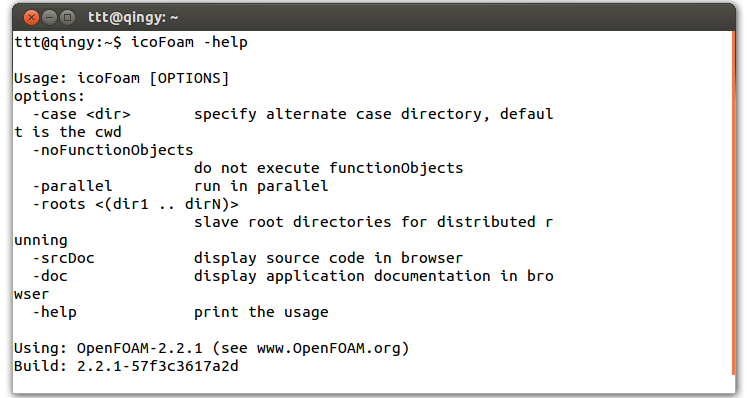
\includegraphics[scale=0.5]{\LocCHonefig/usage.png}
\caption{Usage Message}
\label{usage}
\end{center}  
\end{figure}

\flushleft Now we will set up the working directory and copy the tutorial folder. Follow the steps given below. 
\begin{enumerate}
\item Open up a new terminal and type \textbf{mkdir -p $\$$FOAM$\_$RUN} and press enter
\item Now type \textbf{cp -r $\$$FOAM$\_$TUTORIALS} \textbf{$\$$FOAM$\textunderscore$RUN} and press enter. This will copy the tutorials folder into the run directory.
\end{enumerate}

\flushleft Installation of OpenFOAM using the Debian package is now complete. Similarly you can download it for other linux OS such as Fredora, OpenSUSE.

\section{Installation using Source Code}
Alternate way to install OpenFOAM and Paraview is by Compiling the Source code available under the header of \textbf{Source Pack} Installation on the OpenFOAM website. 
Download the tar files available in \textbf{OpenFOAM.tar.gz} and \textbf{ThirdParty.tar.gz} format. Create a folder in your Home directory by the name OpenFOAM and paste the tar files in that folder and Extract the files in that folder.
Follow the steps given on the OpenFOAM source pack installation page to complete the installation. Since we compile the source code it might take a few hours to complete.

\section{Example Problem - Lid Driven Cavity}
We will solve an problem here by the name Lid Driven Cavity. It is a two dimensional problem where the upper plate moves and other three sides of the plate are fixed / stationary, \ref{lid}. 
The solver we use here is icoFoam which is an Transient solver for incompressible flow.

\begin{figure}[ht]  
\begin{center}  
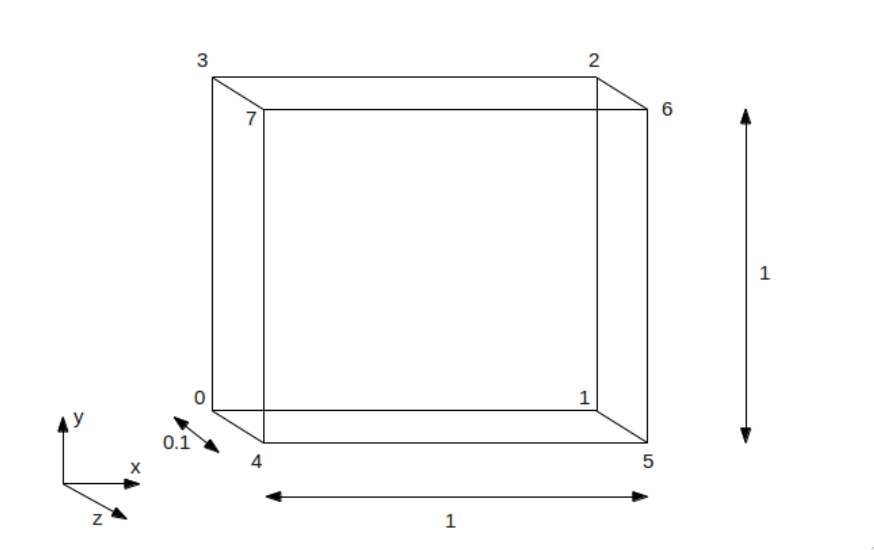
\includegraphics[scale=0.3]{\LocCHonefig/geometry1.png}
\caption{Lid Driven Cavity}
\label{lid}
\end{center}  
\end{figure}

In the terminal type the path given below :\newline

\small{cd OpenFOAM/OpenFOAM-2.3.0/run/tutorials/incompressible/icoFoam/cavity} \newline

\subsection*{Meshing the geometry}
We need to mesh the geometry. This can be done using the blockMesh utility of OpenFOAM. In the command terminal type \textbf{blockMesh} and press $<enter>$ which completes the meshing, Fig \ref{mesh}

\begin{figure}[ht]  
\begin{center}  
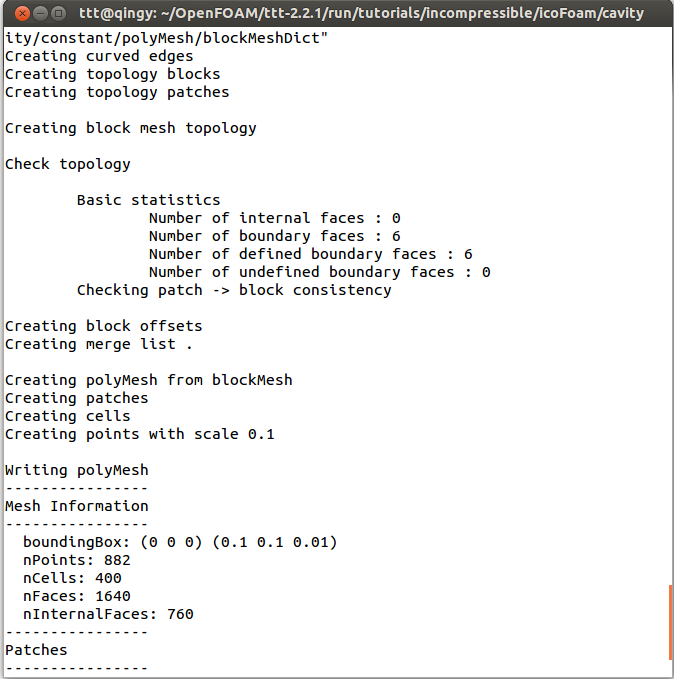
\includegraphics[scale=0.3]{\LocCHonefig/blockMesh.png}
\caption{blockMesh for meshing}
\label{mesh}
\end{center}  
\end{figure}

\newpage

\subsection*{Solving}
Once meshing is done we now run the solver by typing : \\
\center \textbf{icoFoam} \\
\flushleft in the command terminal and press $<enter>$. The iteration running can be seen in the terminal window,Fig \ref{solver}. \newline
\flushleft We have now solved the lid driven cavity case.

\begin{figure}[ht]  
\begin{center}  
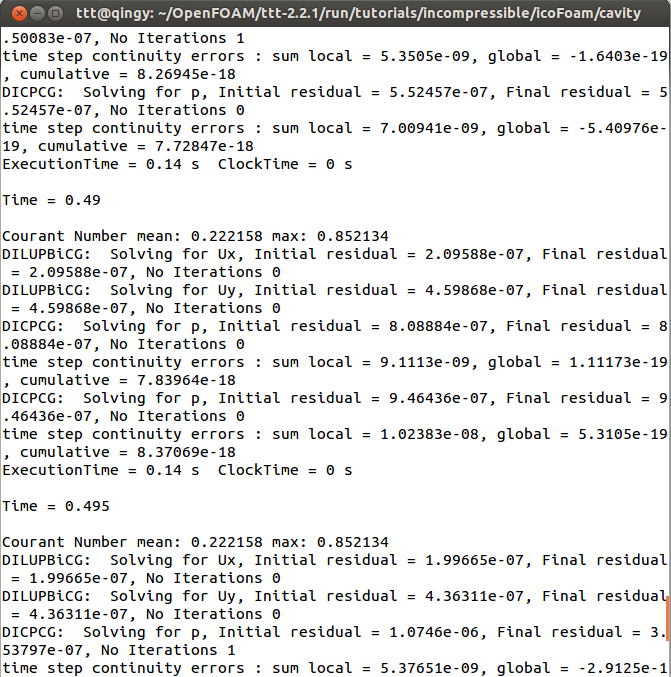
\includegraphics[scale=0.3]{\LocCHonefig/solver.png}
\caption{Iteration on Terminal Window}
\label{solver}
\end{center}  
\end{figure}

\subsection*{Visualization}
To Visualize the results we use Paraview. To open paraview in your terminal type \\
\center \textbf{paraFoam} \\
\flushleft and press $<enter>$. This will open up the paraview window, Fig \ref{pv}.

\begin{figure}[ht]  
\begin{center}  
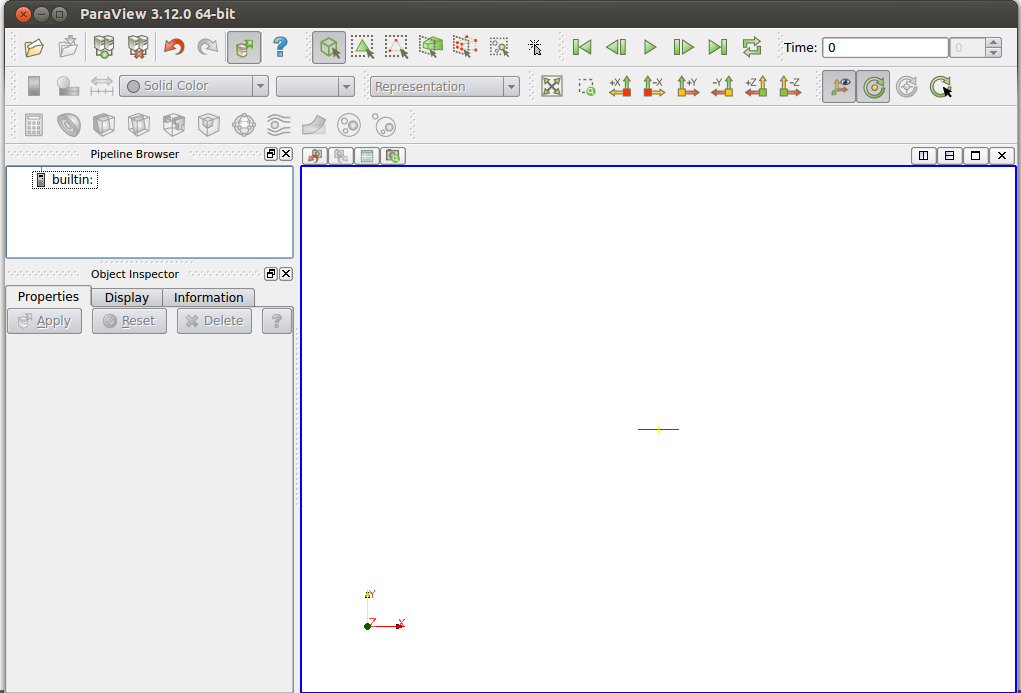
\includegraphics[scale=0.32]{\LocCHonefig/paraview.png}
\caption{Paraview window}
\label{pv}
\end{center}  
\end{figure}

\flushleft Click on the Apply button on the left hand side of the \textbf{Object Inspector} Menu to view the Geometry, Fig\ref{geom}.

\begin{figure}[ht]  
\begin{center}  
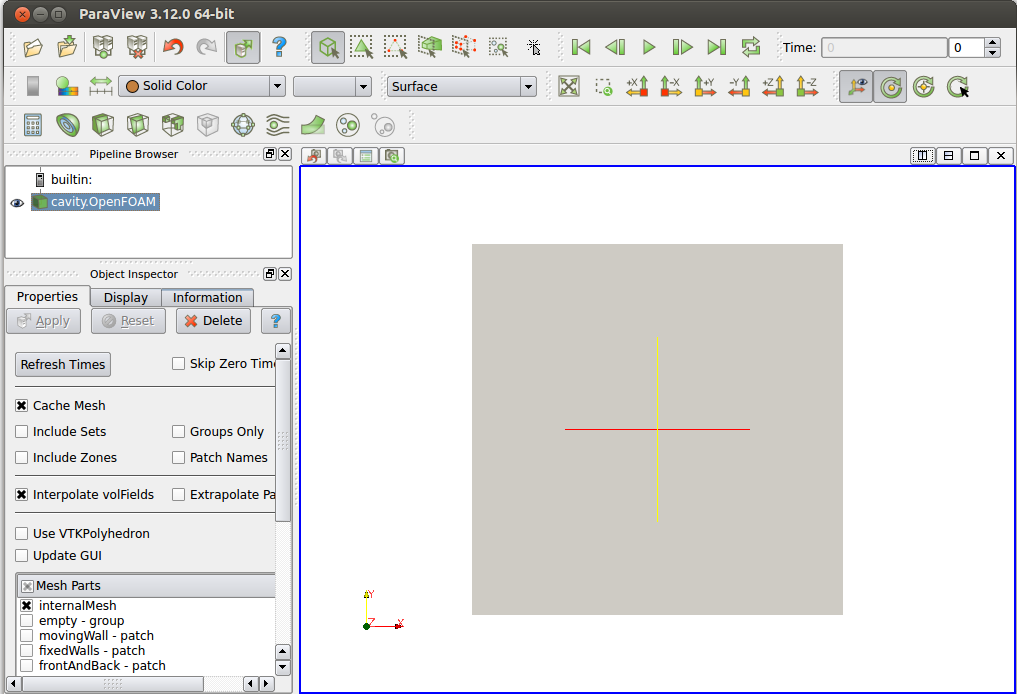
\includegraphics[scale=0.32]{\LocCHonefig/geometry.png}
\caption{Geometry}
\label{geom}
\end{center}  
\end{figure}

\flushleft This brings us to the end of the first chapter. To summaries we have learnt to Install OpenFOAM and Paraview and ran a test example. 
The next chapter will cover about creating simple geometry in OpenFOAM.
